\documentclass[border=10pt]{standalone}
\usepackage{pgfplots}
\usepgfplotslibrary{colormaps}
\pgfplotsset{trig format plots=rad}
\begin{document}
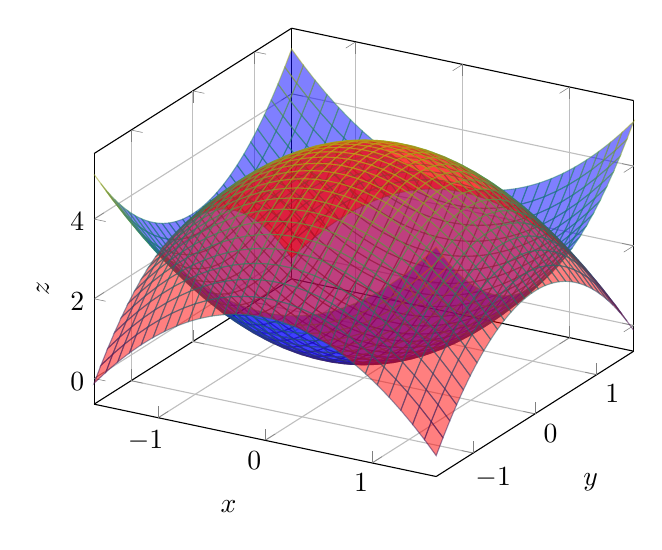
\begin{tikzpicture}
\begin{axis}[
    view={30}{30},
    xlabel={$x$},
    ylabel={$y$},
    zlabel={$z$},
    colormap/viridis,
    grid=major,
    domain=-2:2,
    y domain=-2:2,
    samples=30,
    clip=false
]
    % Surface 1: z = x^2 + y^2
    \addplot3[surf, opacity=0.5, blue, domain=-1.6:1.6, y domain=-1.6:1.6] {x^2 + y^2};
    
    % Surface 2: z = 5 - x^2 - y^2
    % Note: The domain for Z2 should be restricted to the intersection for a cleaner look, 
    % but standard surface plots show the whole function.
    % However, to show the "enclosed" part, we should ideally restrict the domain.
    % The intersection is r^2 = 2.5, so r ~ 1.58.
    \addplot3[surf, opacity=0.5, red, domain=-1.6:1.6, y domain=-1.6:1.6] {5 - x^2 - y^2};

\end{axis}
\end{tikzpicture}
\end{document}
